% Asset ID: FAS2WorkEnergyAndPowerTikZ-001
% Rough-plane force and energy diagram
\documentclass[tikz,border=8pt]{standalone}
\usepackage{tikz}
\usepackage{amsmath}
\usetikzlibrary{arrows.meta,angles,quotes,calc,decorations.pathreplacing}
\begin{document}
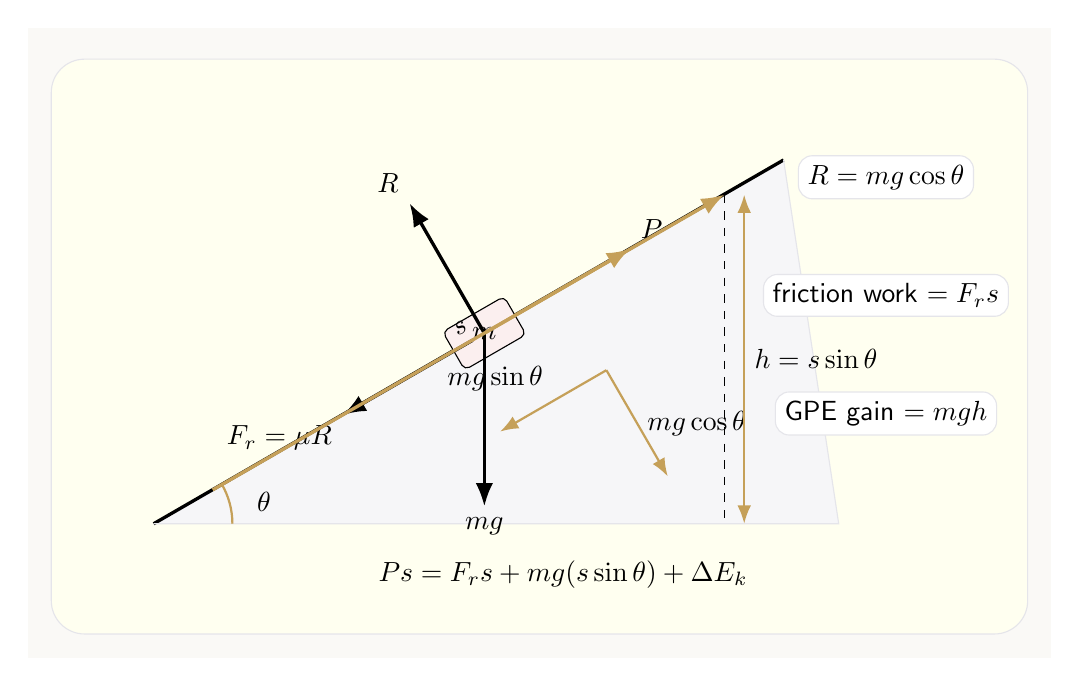
\begin{tikzpicture}[>=Latex, every node/.style={font=\sffamily}, force/.style={->, very thick}]
\definecolor{Canvas}{HTML}{FAF9F6}\definecolor{Paper}{HTML}{FFFFF0}\definecolor{LineSoft}{HTML}{E5E5EA}\definecolor{Accent}{HTML}{C5A059}\definecolor{SoftPink}{HTML}{FBEFEF}\definecolor{Text}{HTML}{2C2C2E}
\fill[Canvas] (-1,-1) rectangle (12,7);
\draw[LineSoft, rounded corners=12pt, fill=Paper] (-.7,-.7) rectangle (11.7,6.6);
\coordinate (A) at (.6,.7); \coordinate (B) at (8.6,5.32); \coordinate (C) at (9.3,.7); \coordinate (O) at (4.8,3.12);
\fill[LineSoft!35] (A)--(B)--(C)--cycle; \draw[very thick] (A)--(B); \draw[LineSoft] (A)--(C)--(B);
\draw[Accent, thick] (1.6,.7) arc[start angle=0,end angle=30,radius=1]; \node at (2,.98) {$\theta$};
\begin{scope}[shift={(O)}, rotate=30] \draw[fill=SoftPink, rounded corners=2pt] (-.45,-.28) rectangle (.45,.28); \node {$m$}; \end{scope}
\draw[force, draw=Accent] (O)--++(1.85,1.07) node[above right] {$P$};
\draw[force] ($(O)+(-.15,-.09)$)--++(-1.65,-.95) node[below left] {$F_r=\mu R$};
\draw[force] (O)--++(-.95,1.65) node[above left] {$R$};
\draw[force] (O)--++(0,-2.2) node[below] {$mg$};
\draw[->, thick, draw=Accent] (6.35,2.65)--++(-1.35,-.78) node[midway, above left] {$mg\sin\theta$};
\draw[->, thick, draw=Accent] (6.35,2.65)--++(.78,-1.35) node[midway,right] {$mg\cos\theta$};
\draw[->, very thick, draw=Accent] (1.35,1.13)--(7.85,4.88) node[midway,above,sloped] {$s$};
\draw[dashed] (7.85,4.88)--(7.85,.7); \draw[<->, thick, draw=Accent] (8.1,.7)--(8.1,4.88) node[midway,right] {$h=s\sin\theta$};
\node[draw=LineSoft, fill=white, rounded corners=5pt, align=left] at (9.9,5.1) {$R=mg\cos\theta$};
\node[draw=LineSoft, fill=white, rounded corners=5pt, align=left] at (9.9,3.6) {friction work $=F_rs$};
\node[draw=LineSoft, fill=white, rounded corners=5pt, align=left] at (9.9,2.1) {GPE gain $=mgh$};
\node at (5.8,.05) {$Ps=F_rs+mg(s\sin\theta)+\Delta E_k$};
\end{tikzpicture}
\end{document}
